\section{Problem Statement}

The following definition is an extended version of HIN \cite{sun2011pathsim} for the dynamic network case.

\begin{definition}[Dynamic heterogeneous information network]
A dynamic heterogeneous information network (DHIN) is a directed graph $G$ = ($V$, $E$) with a node type mapping function $\phi: V \rightarrow \mathcal{A}$ and a link type mapping function $\psi: E \rightarrow \mathcal{R}$, where $V$, $E$, $\mathcal{A}$, and $\mathcal{R}$ denote sets of nodes, links, node types, and relation types. Each node $v \in V$ belongs to a node type $\phi(v) \in \mathcal{A}$, each link $e \in E$ belongs to a relation $\psi(e) \in \mathcal{R}$, and $|\mathcal{A}| > 1$ and $|\mathcal{R}| > 1$. Also each edge $e = (u, v, t)$ is a temporal edge from a vertex $u$ to a vertex $v$ at time $t$. 
$\Box$ 

\end{definition}

%\begin{example}
The DBLP bibliographic network\footnote{\url{http://dblp.uni-trier.de/db/}} is an example of a DHIN, containing different types of nodes such as papers, authors, topics, and publication venues, with publication links associated with date. Another example is the Twitter social network with nodes of types posted tweets, users, topics, and hashtags and time window associated with these tweets. %$\Box$
%\end{example}

In the context of a heterogenous network, a \textit{relation} can be in the form of a \textit{direct link} or an \textit{indirect link}, where an indirect link is a sequence of direct links in the network. Thus, two nodes might not be directly connected, however they might be connected considering the semantic of a sequence of links of different types. In this work, we use the terms \textit{relationship prediction} and \textit{link prediction} interchangeably referring to predicting whether two nodes will be connected in future via a \textit{sequence of relations} in the graph, where the \textit{length} of a sequence is greater than or equal to one. For instance in a bibliographic network a direct link exist between an author and a paper he wrote, and an indirect link exist between him and his co-authors through the paper, which they wrote together.

In order to better understand different types of nodes and their relation in a network, the concept of \textit{network schema} \cite{sun2011pathsim} is used. A network schema is a meta structure graph that summarizes a HIN and is formally defined as bellow.

\begin{definition}[Network schema]
For a heterogeneous network $G=(V,E)$, the network schema $S_G=\mathcal{(A,R)}$ is a directed meta graph where $\mathcal{A}$ is the set of node types in $V$ and $\mathcal{R}$ is the set of relation types in $E$.  $\Box$
\end{definition}

%\begin{example}
Figure \ref{schema} shows the network schema for the DBLP bibliographic network with $\mathcal{A}$=\{\textit{Author}, \textit{Paper}, \textit{Venue}, \textit{Topic}\}. %$\Box$
%\end{example}
In this paper, we refer to different types of nodes in the DBLP bibliographic network with abbreviations $P$ for paper, $A$ for author, $T$ for topic, and $V$ for venue. 

\begin{figure}[t]
  \centering
      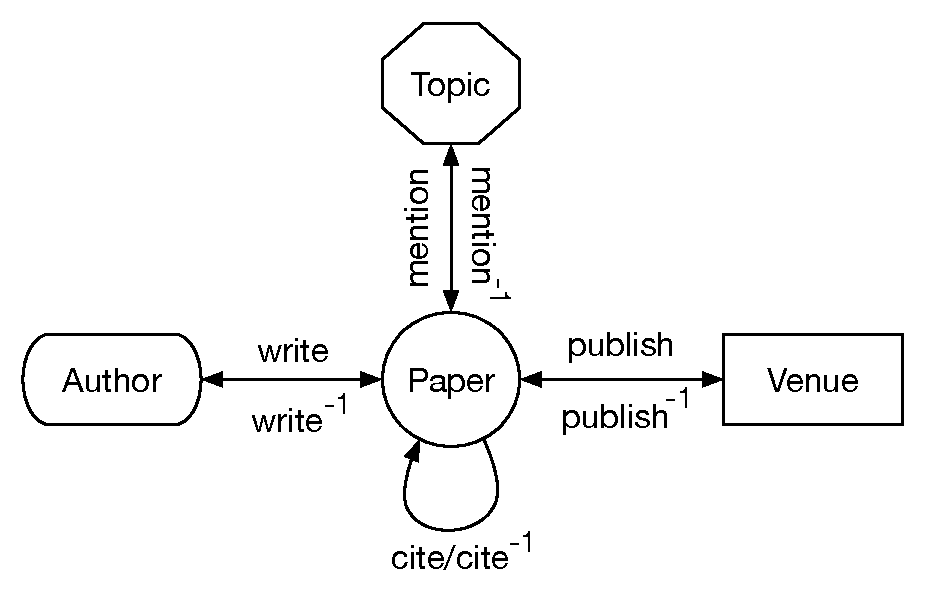
\includegraphics[trim = 0mm 10mm 0mm 0mm,width=0.42\textwidth]{figs/schema.pdf}
  \caption{Network schema for DBLP network.}\label{schema}
\end{figure}

%\subsection{Meta path-based topology}

Similar to the notion of network schema that provides a meta structure for the network, a \textit{meta path} \cite{sun2011pathsim} provides a meta structure for paths between different nodes in the network. 

\begin{definition}[Meta path]
A meta path $P$ is a path in a network schema graph $S_G = (\mathcal{A,R})$, denoted by $P(A_1,A_{n+1}) = A_1 \xrightarrow{R_1} A_2... \xrightarrow{R_n} A_{n+1}$, as a sequence of links between node types, which defines a composite relationship between a node of type $A_1$ and one of type $A_{n+1}$, where $A_i \subseteq \mathcal{A}$ and $R_i \subseteq \mathcal{R}$. $\Box$
\end{definition}

The \textit{length} of a meta path is the number of relations in it. Note that given two node types $A_i$ and $A_j$, there may exist multiple meta paths of different lengths between them. We call a path $p = (a_1a_2...a_{n+1})$ a \textit{path instance} of a meta path $P = A_1-A_2... -A_{n+1}$ if $p$ follows $P$ in the corresponding HIN, i.e., for each node $a_i$ in $p$, we have $\phi(a_i)=A_i$. The co-author relationship in DBLP can be described with the meta path $A\xrightarrow{write}P\xrightarrow{write^{-1}}A$ or in short \textit{A--P--A}. Paths in thick solid lines in Figure \ref{sampleNetwork} correspond to \textit{A--P--V--P--A} meta paths between \textit{Max} and \textit{Ada}, indicating they published in the same venue, such as \textit{Max--P1--KDD--P3--Ada}. %$\Box$
%\end{example}
Each meta path indicates a different semantic and defines a unique topology representing a special relation. The relationship between two authors are different in meaning when they are co-authors (\textit{A--P--A}) versus one citing another's paper (\textit{A--P--P--A}).

\begin{figure}[t]
  \centering
      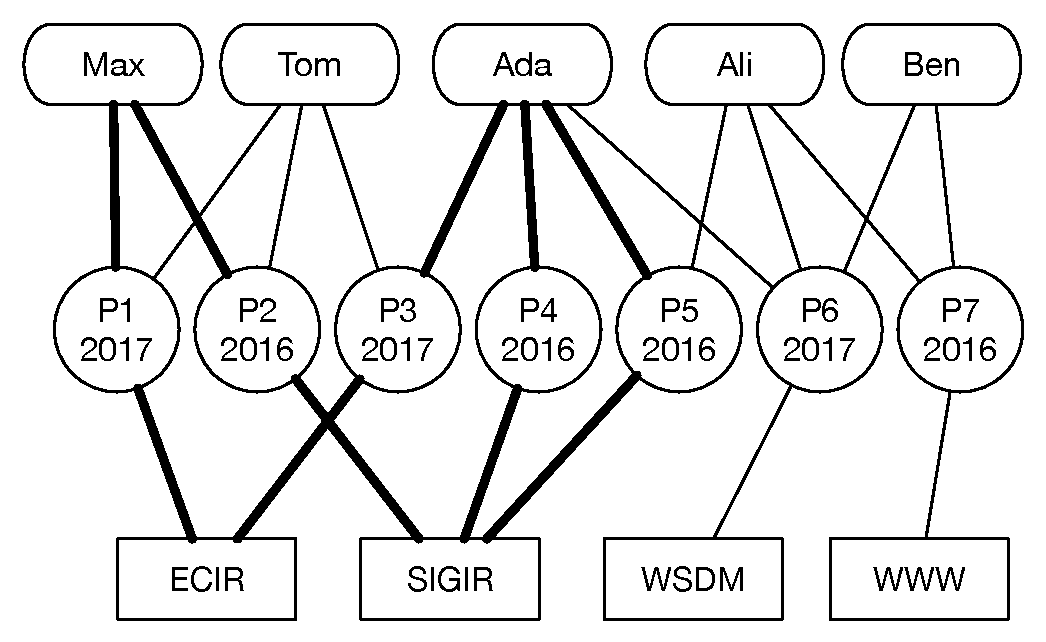
\includegraphics[width=0.4\textwidth]{figs/exampleSocialNetwork.pdf}
  \caption{An example of \textit{A--P--V--P--A} meta paths between two authors Max and Ada.}\label{sampleNetwork}
\end{figure}

\textbf{Meta Path-based Similarity Measures.} Given a meta path $P = (A_i,A_j)$ and a pair of nodes $a$ and $b$ that $\phi(a)=A_i$ and $\phi(b)=A_{j}$, several \textit{similarity measures} can be defined between $a$ and $b$ based on the path instances of $P$. Examples of such similarity or proximity measures in a HIN are \textit{path count} \cite{sun2011pathsim,sun2011ASONAM}, \textit{PathSim} \cite{sun2011pathsim} or \textit{normalized path count} \cite{sun2011ASONAM}, \textit{random walk} \cite{sun2011ASONAM}, and \textit{HeteSim} \cite{shi2014hetesim}. Given a meta path $P$ a source node $a$ and a target node $b$, path count measures the number of path instances between $a$ and $b$ following $P$, and can be calculated by multiplying adjacency matrices of relations in $P$ \cite{sun2011ASONAM}, and random walk is the probability of the random walk that starts from $a$ and ends with $b$ following $P$. More discussion about these similarity measures can be found in \cite{shi2014hetesim,sun2011ASONAM,sun2011pathsim}. Without loss of generality, in this work we use the path count as the default measure. For example given the meta path \textit{A--P--V--P--A} and the HIN in Figure \ref{sampleNetwork}, $PC(Max,Ada)$=3 and $PC(Max,Tom)$=3. 

We now formally define the problem that we target in this work as follows:

\begin{definition}[\textbf{Relationship prediction problem}]\label{problemdef}
Given a DHIN graph $G$ at time $t$, and a target relation meta path $P(A_i,A_j)$ between nodes of type $A_i$ and $A_j$, we aim to predict the existence of a path instance of $P$ between two given nodes of types $A_i$ and $A_j$ at time $t+1$. $\Box$
 \end{definition}




%By checking the existing topological features defined in homogeneous networks, we can find that both the neighbor set-based features and path-based features can be generalized in heterogeneous information networks, by considering paths following different meta paths. For example, if we treat each type of neighbors separately and extend the immediate neighbors to n-hop neighbors (i.e., the distance between one object and its neighbors are n), the common neighbor feature between two authors is then becoming the count of paths between the two authors following different meta paths. For path-based features, such as Katz, it can be extended as a combination of paths following different meta paths. 


%\begin{table*}[h]
%\centering
%\caption{Notations and their description.\amin{may remove for space limit.}}
%\scriptsize
%\label{table_notations}
%\begin{tabular}{|c|l|} \hline
%\textbf{Notation} & \textbf{Description} \\ \hline
%
%$\mathcal{A}, \mathcal{R}$  &  Types of objects and relations \\ \hline
%$\mathcal{P}$, $p$  & Meta path and path \\ \hline
%$k$ & The dimension of latent features \\ \hline
%$G_\tau$ & Graph $G$ at time $\tau$  \\ \hline
%$\hat{G}_\tau$ & Predicted graph $G$ at time $\tau$  \\ \hline
%$Z_\tau$ & low rank $k$-dimensional latent space representation matrix for $G_\tau$ \\ \hline
%
%\end{tabular}
%\end{table*}

